\section{Calibración}

\par
La compañía SIGCSA utiliza para sus servicios termómetros calibrados, esto garantiza que sus equipos muestran mediciones dentro de estándar aceptable. Uno de los aspectos fundamentales de la medición de la temperatura es la calibración de esta; ya que, no todos los sistemas trabajan con los mismos estándares. 

\subsection{¿Que es Calibración?}

\par 
La palabra "calibración" tiene diferentes significados dependiendo de la industria o el entorno en el que se utiliza. En la industria de prueba y medición, la calibración tiene un significado específico, que, en un nivel básico, es el acto de comparar un dispositivo bajo prueba (DUT por sus siglas en ingles) de un valor desconocido con un estándar de referencia de un valor conocido. Una persona típicamente realiza una calibración para determinar el error o verificar la exactitud del valor desconocido del DUT. Como ejemplo básico, puede realizar una calibración midiendo la temperatura de un termómetro DUT en agua en el punto de ebullición conocido (100 grados Celsius) para conocer el error del termómetro. Debido a que la determinación visual del momento exacto en que se alcanza el punto de ebullición puede ser impreciso, usted puede lograr un resultado más preciso colocando un termómetro de referencia calibrado, de un valor conocido preciso, en el agua para verificar el termómetro DUT\cite{calibracion-fluke1}.

\par \noindent
Un siguiente paso lógico que puede ocurrir en un proceso de calibración puede ser ajustar o realzar el instrumento para reducir el error de medición. Técnicamente, el ajuste es un paso separado de la calibración\cite{calibracion-fluke}.

\par \noindent
Ahora ¿cómo llegamos a estándares de medición de valores conocidos contra los cuales calibramos nuestros dispositivos bajo prueba? Para la respuesta, pasamos al Sistema Internacional de Unidades, abreviado "SI". 

\subsubsection{Sistema Internacional de Unidades (SI) \cite{calibracion-fluke}}

\par \noindent
El SI consta de siete unidades base que son:

\begin{itemize}
	\item  Metro (m): Es la longitud del camino recorrido por la luz en el vacío durante un intervalo de tiempo de 1/299 792 458 de segundo.
	
	\item Kilogramo (kg): Es la unidad de masa; es igual a la masa del prototipo internacional del kilogramo. Actualmente esta siendo redefinida utilizando la balanza de Kibble.
	
	\item Segundo (s): Es la duración de 9 192 631 770 períodos de la radiación correspondiente a la transición entre los dos niveles hiperfinos del estado fundamental del átomo de cesio 133.
	
	
	\item Ampere (A): Es la corriente constante que, si se mantiene en dos conductores paralelos rectas de longitud infinita, de sección transversal circular insignificante, y se coloca a 1 m de distancia en el vacío, produciría entre estos conductores una fuerza igual a 2 x 10-7 newton por metro de longitud.
	
	\item Kelvin (K): Unidad de temperatura termodinámica, es la fracción 1 / 273.16 de la temperatura termodinámica del punto triple del agua.
	
	\item Mol (mol): Es la cantidad de sustancia de un sistema que contiene tantas entidades elementales como átomos hay en 0.012 kilogramos de carbono 12.
	
	\item Candela (cd): Es la intensidad luminosa, en una dirección dada, de una fuente que emite radiación monocromática de frecuencia 540 x 1012 hercios y que tiene una intensidad radiante en esa dirección de 1/683 vatios por estereorradián.
\end{itemize}

\par \noindent
Ahora que tenemos los estándares de referencia SI, ¿cómo los compartimos de manera eficiente y económica con el mundo?

\subsubsection{Piramide de Trazabilidad de Calibración \cite{calibracion-fluke}}

\begin{figure}[H]
	\centering
	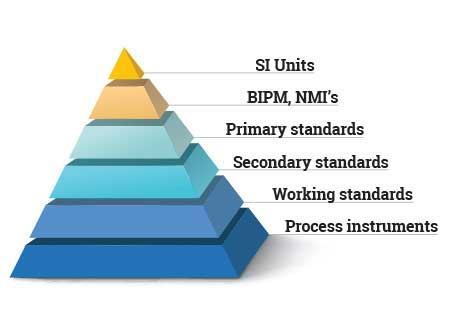
\includegraphics[width=0.8\textwidth]{calibracion1.jpg}
	\caption{Pirámide de Trazabilidad de Calibración}
\end{figure}

\par 
El SI se encuentra en la parte superior de una pirámide de calibración donde el BIPM ayuda a pasar el SI a todos los niveles de uso dentro de los países para fomentar el descubrimiento científico y la innovación, así como la fabricación industrial y el comercio internacional.

\par \noindent 
Justo debajo del nivel SI, el BIPM (Bureau International des Poinds et Measures por sus siglas en francés), es organización intergubernamental a través de la cual los Estados miembros actúan juntos
en asuntos relacionados con la ciencia de medición y los estándares de medición, trabaja directamente con los Institutos Nacionales de Metrología (NMIs por sus siglas en inglés) de los estados miembros o países para facilitar la promoción de la SI dentro de esos países.

\par \noindent
El NMI de los Estados Unidos de América es el National Institute of Standarts and Technology (NIST por sus siglas en inglés); mientras que, el NMI de Panamá es el Centro Nacional de Metrología de Panamá (CENAMEP).

\clearpage

\par \noindent
Debido a que no es economico, eficiente o incluso posible para todos en un país trabajar directamente con su NMI, los estándares de calibración de NMI se utilizan para calibrar los estándares o instrumentos de calibración primarios; los estándares primarios luego se usan para calibrar estándares secundarios; los estándares secundarios se utilizan para calibrar estándares de trabajo; y los estándares de trabajo se usan para calibrar instrumentos de proceso. De esta manera, las referencias a los estándares SI pueden transmitirse de manera eficiente a través de la NMI a la pirámide de calibración, a la industria según sea necesario.

\subsubsection{Acreditación de Calibración \cite{calibracion-fluke}}

\par 
Cuando se realizan calibraciones, es importante poder confiar en el proceso por el cual se realizan. La acreditación de calibración brinda esa confianza. La acreditación le da confianza al propietario del instrumento de que la calibración se ha realizado correctamente.

\par \noindent
La acreditación de calibración significa que se ha revisado un proceso de calibración y se ha encontrado que cumple con los requisitos de metrología técnica y de calidad aceptados internacionalmente. ISO / IEC 17025 es la norma de calidad de metrología internacional a la cual los laboratorios de calibración están acreditados.

\par \noindent
Los acuerdos internacionales garantizan que una vez que se acredita un proceso de calibración en un país, las calibraciones provenientes de ese proceso pueden aceptarse en todo el mundo sin ningún requisito de aceptación técnica adicional.

\subsubsection{Disciplinas de la Calibración \cite{calibracion-fluke}}

\par 
Hay muchas disciplinas de calibración, cada una con diferentes tipos de calibradores y referencias de calibración. Para tener una idea de los tipos de calibradores e instrumentos que están disponibles. Las disciplinas comunes de calibración incluyen, pero no están limitadas a: electrica, radio frecuencia, temperatura, humedad, presión, flujo de aire, dimensional, tiempo.

\par \noindent
La disciplina de calibración en la cual estamos interesados para evaluar nuestro prototipo es la calibración de temperatura.

\clearpage



\subsection{¿Qué es Calibración de Temperatura?}

\par 
La calibración de temperatura se refiere a la calibración de cualquier dispositivo utilizado en un sistema que mide la temperatura. Generalmente hablamos del sensor de temperatura, que es típicamente un termómetro de resistencia de platino (PRT o PT-100), termistor o termopar. Las lecturas de estos termómetros se realizan mediante dispositivos de "lectura de termómetro" que miden sus salidas eléctricas y las convierten a temperatura de acuerdo con la Escala de temperatura internacional de 1990 (ITS-90).
Los termómetros suelen calibrarse colocándolos en un entorno de temperatura estable (fuente de calor) y comparando su salida con la de un "termómetro de referencia" calibrado o "termómetro estándar" \cite{temperatura-fluke}. 

\par \noindent
Por lo general las categorías generales de fuentes de calor son: fuentes de calor industriales (baño-seco, micro-baños, etc.) para uso en el campo; baños de fluidos y hornos termoeléctricos para uso en laboratorio; y células de punto fijo para calibraciones con estandares primarios.

\subsubsection{Campo, Laboratorio y Punto fijo \cite{temperatura-fluke}}

\paragraph{Calibración de Temperatura en Campo}
Tambien llamado calibración de temperatura "industrial" o "portátil", se aplica a los termómetros que se prueban fuera del entorno de laboratorio, generalmente a precisiones que van desde 5 ° C a 0,5 ° C. Pozos secos, pozos de metrología, micro-baños, objetivos de IR y otras fuentes de calor portátiles proporcionan temperaturas estables, mientras que las lecturas de termómetros portátiles y los estándares de termómetros pueden proporcionar temperaturas de referencia más allá de las disponibles directamente de la fuente de calor.

\paragraph{Calibración Secundaria o de Laboratorio}
Se refiere a la calibración de PRT o PT-100 de grado de referencia, termistores de precisión y termopares de metal noble. Baños de temperatura ultraestables y uniformes y hornos horizontales (para las altas temperaturas que necesitan los termopares) se usan junto con los termómetros de referencia SPRT y las lecturas de termómetros de alta precisión. Dichos sistemas pueden proporcionar precisiones de calibración de 0.5 ° C a 0.02 ° C.

\paragraph{Calibración Primaria o de Punto fijo} 
Utiliza celdas de punto fijo, como el punto triple de agua, que proporciona una temperatura extremadamente precisa y repetible cuando se "realizan" correctamente, normalmente en un entorno de laboratorio. Dichos sistemas se utilizan para calibrar los SPRT y los termopares de metal noble y pueden tener una precisión de 0.001 ° C.

\subsubsection{Equipos utilizados para la Calibración de Termometros}

\par 
La calibración de termometros es realizada utilizando el sistema verdadero de calibración donde el equipo a calibrar no debe estar previamente calibrado y llamamos termómetro a calibrar, al termometro (PRT, termistor o termopar) y el indicador de temperatura en conjunto.

\par \noindent
Se necesita para realizar la calibración de un termómetro: un termómetro de referencia o patrón, una fuente de temperatura, las condiciones ambientales adecuadas y el termómetro a calibrar.

\par \noindent
La norma ISO 17025:2005 indica que el termómetro de referencia debe ser más preciso, que el termómetro a calibrar; sin embargo, no especifica que superior debe ser con respecto a el termómetro a calibrar. Fluke Calibration, empresa norteamericana con acreditaciones ISO 17025 en laboratorios primarios y secundarios de temperatura, recomienda que un termómetro de referencia aceptable debe por lo menos ser 3 veces mejor, que el termómetro a calibrar.

\begin{figure}[H]
	\centering
	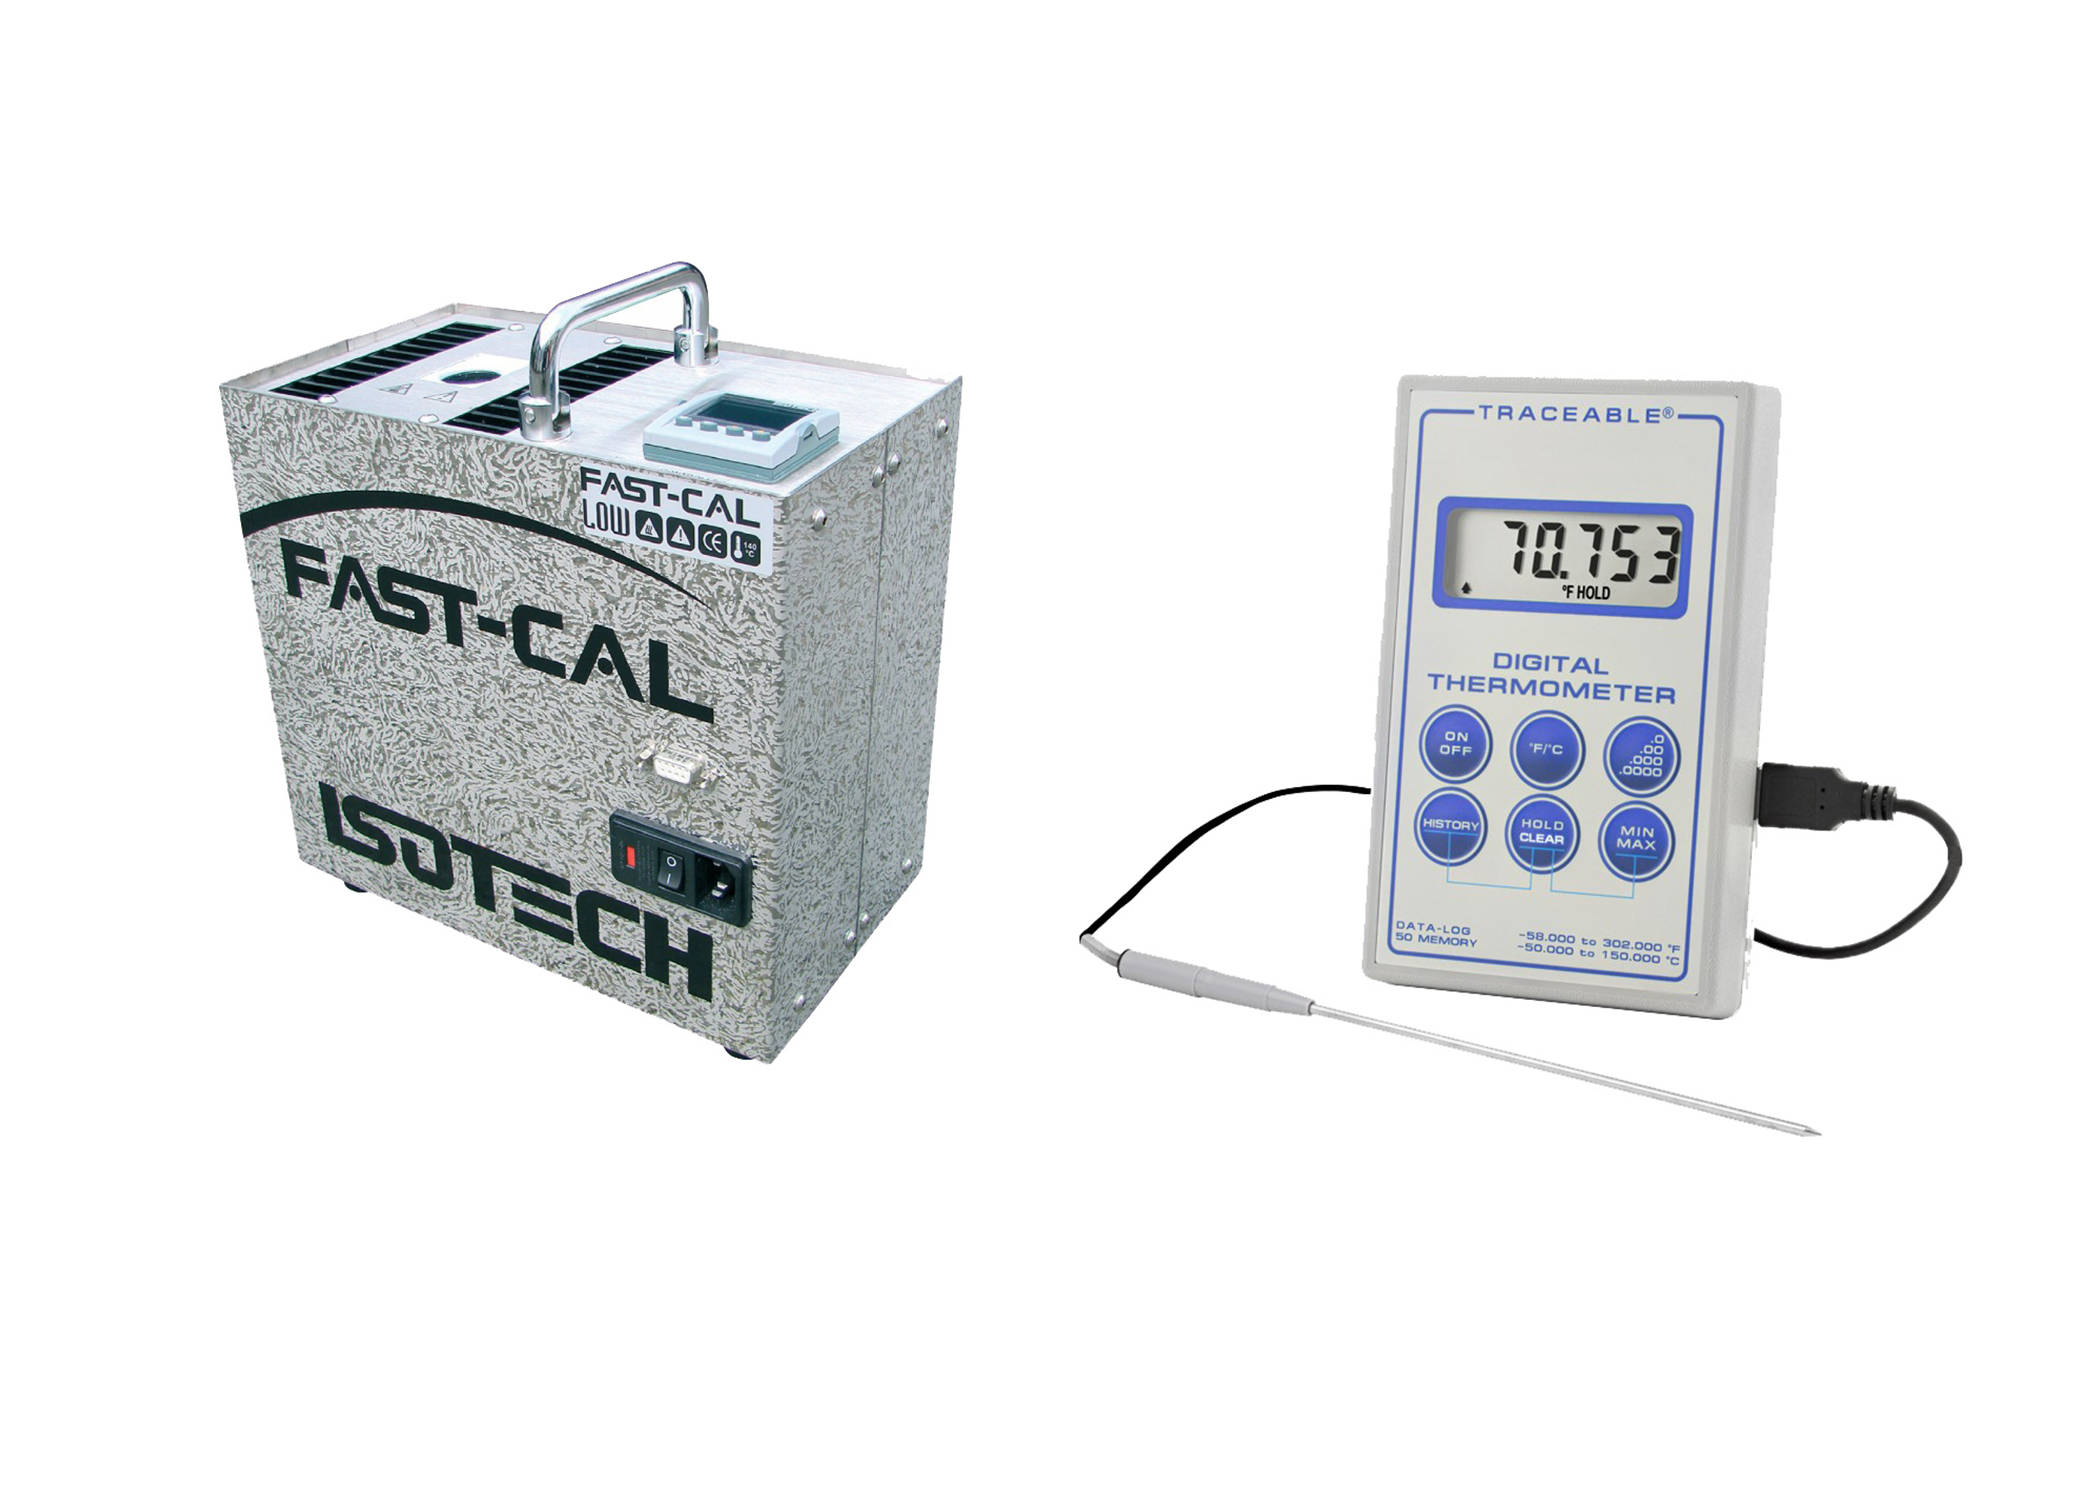
\includegraphics[width=0.6\textwidth]{caltemperatura1.png}
	\caption{Bloque de baño seco (Izquierda) y termómetro de referencia utilizado en SIGCSA (Derecha)}
\end{figure}

\par \noindent
La fuente de temperatura puede ser de 3 tipos: celdas de punto fijo, baños de fluido o calibradores de bloque seco.
Cada fuente brinda sus ventajas y desventajas. Debido a que SIGCSA realiza calibraciones en campo se utilizarán los bloques de baño seco estos nos permiten una excelente precisión en la temperatura seleccionada, es portátil y no requiere unas condiciones ambientales muy estrictas.
Adicional estos instrumentos incluyen indicadores de temperatura que son calibrados con estándares primarios.

\par \noindent
Los equipos que vayamos a utilizar dependeran del tipo de calibración de temperatura que vayamos a realizar. Los equipos utilizados en SIGCSA son excelentes para realizar calibraciones de temperatura en campo y dispositivos de grado industrial; sin embargo, si queremos realizar calibraciones de estandares secundarios o primarios, se necesitarian equipos de mayor precisión a los de grado industrial.

\begin{figure}[H]
	\centering
	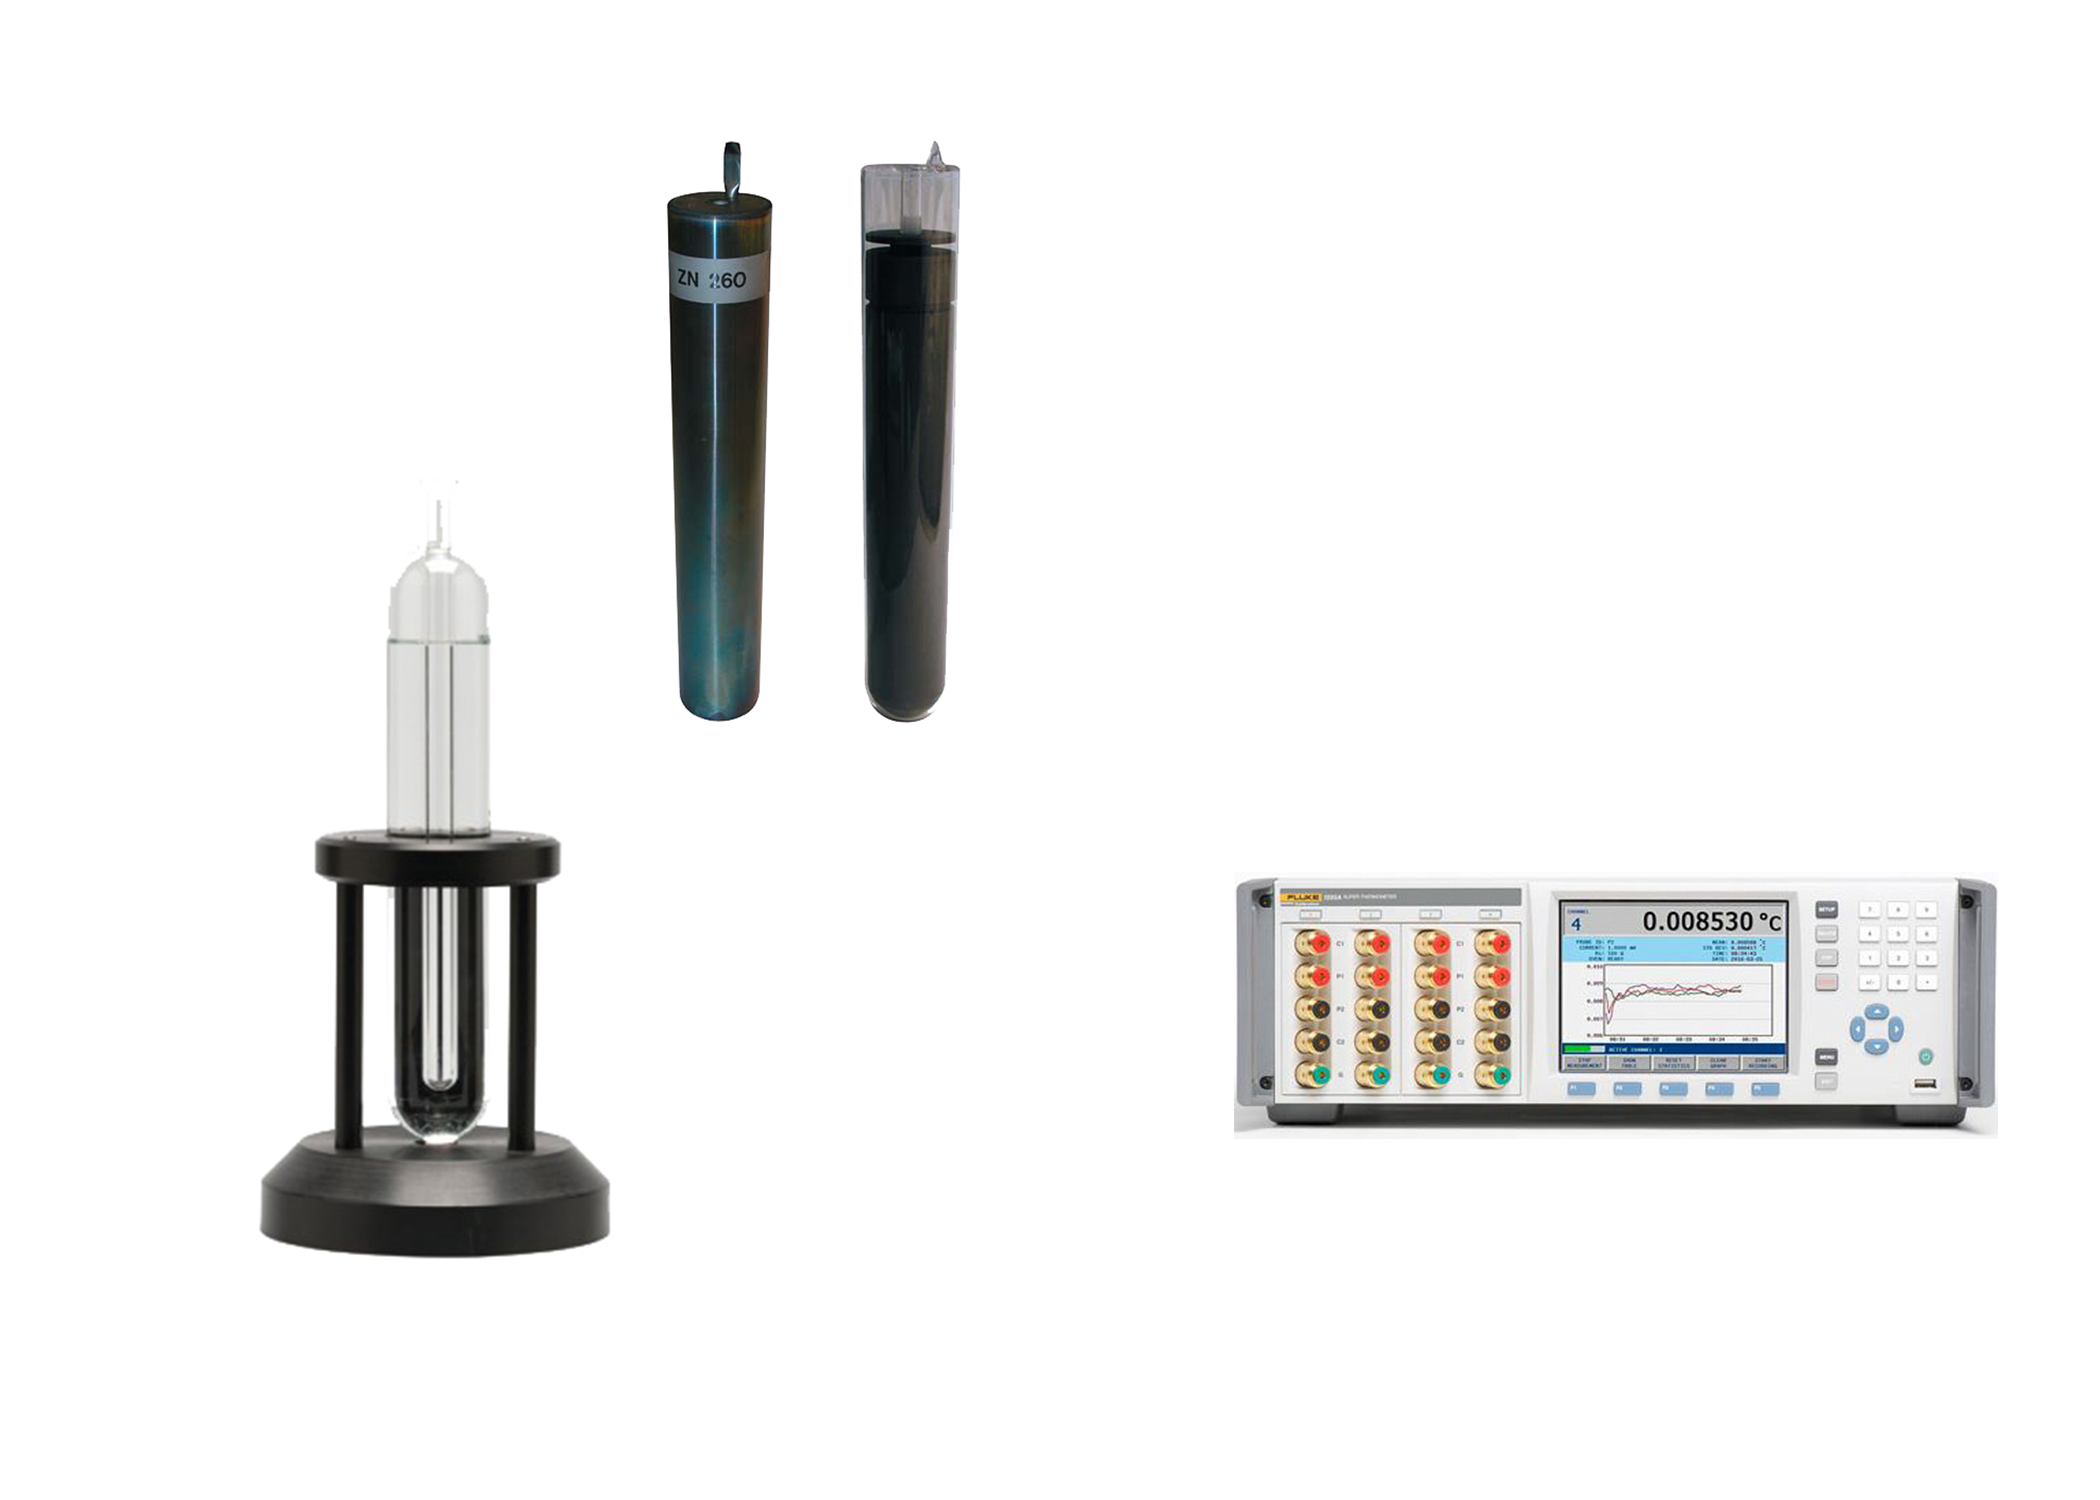
\includegraphics[width=\textwidth]{caltemperatura2.png}
	\caption{Celdas de punto fijo ITS-90 y Fluke Supertermómetro 1594A, ambos utilizados para calibraciones de estándares primarios.}
\end{figure}





\par \noindent
Como hemos percatado la disciplina de la calibración se encuentra atada a las normas de calidad ISO. Es necesario investigar sobre estas normas de calidad; ya que, nos darían una guía de como elaborar y calibrar nuestro prototipo.
